\def \tweite {10.1cm}
%\section*{REST-API}
\subsection*{Query-Methoden}
\textbf{POST \texttt{/queries/post}}
\begin{table}[h!]
\begin{tabular}{| c | p{\tweite} | l |}
\hline
	\textbf{Parameter} & \textbf{Beschreibung} &  \\
\hline \hline
 	\texttt{q} & Suchbegriff & verpflichtend \\
\hline
\end{tabular}
\end{table}
\newline
Legt einen noch nicht existierenden Suchbegriff in der Datenbank an.
\newline
 \newline
\textbf{POST \texttt{/queries/postPriority}}
\begin{table}[h!]
\begin{tabular}{| c | p{\tweite} | l |}
\hline
	\textbf{Parameter} & \textbf{Beschreibung} &  \\
\hline \hline
 	\texttt{id} & ID eines vorhandenen Suchbegriffs & verpflichtend \\
\hline
 	\texttt{p} & Neue Priorität für den angegebenen Suchbegriff & verpflichtend \\
\hline
\end{tabular}
\end{table}
\newline
Ändert die User-Priorität für einen Suchbegriff.
\newline
 \newline
\textbf{POST \texttt{/queries/postActiveFlag}}
\begin{table}[h!]
\begin{tabular}{| c | p{\tweite} | l |}
\hline
	\textbf{Parameter} & \textbf{Beschreibung} &  \\
\hline \hline
 	\texttt{id} & ID eines vorhandenen Suchbegriffs & verpflichtend \\
\hline
 	\texttt{active} & True oder false, je nachdem ob der Suchbegriff für den Daemon aktiv oder inaktiv sein soll (verpflichtend) & verpflichtend \\
\hline
\end{tabular}
\end{table}
\newline
Aktiviert oder deaktiviert einen Suchbegriff für den Daemon.
\newpage

\noindent
\textbf{GET \texttt{/queries/byid}}
\begin{table}[h!]
\begin{tabular}{| c | p{\tweite} | l |}
\hline
	\textbf{Parameter} & \textbf{Beschreibung} &  \\
\hline \hline
 	\texttt{id} & ID eines Suchbegriffs & verpflichtend \\
\hline
\end{tabular}
\end{table}
\newline
Liefert den durch die ID spezifizierten Suchbegriff aus der Datenbank zurück, falls vorhanden.

\noindent
\textbf{GET \texttt{/queries/bystring}}
\begin{table}[h!]
\begin{tabular}{| c | p{\tweite} | l |}
\hline
	\textbf{Parameter} & \textbf{Beschreibung} &  \\
\hline \hline
 	\texttt{q} & Suchbegriff & verpflichtend \\
\hline
\end{tabular}
\end{table}
\newline
Liefert den angegebenen Suchbegriff aus der Datenbank (inklusive ID) zurück, falls vorhanden.

\begin{figure}[h!]
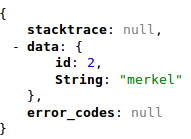
\includegraphics[scale=0.6]{Bilder/RestApi/queriesByString.png}
\end{figure}

\noindent
\textbf{GET \texttt{/queries/contains}}
\begin{table}[h!]
\begin{tabular}{| c | p{\tweite} | l |}
\hline
	\textbf{Parameter} & \textbf{Beschreibung} &  \\
\hline \hline
 	\texttt{q} & Suchbegriff & verpflichtend \\
\hline
\end{tabular}
\end{table}
\newline
Liefert zurück, ob der angegebene Suchbegriff in der Datenbank vorhanden ist.

\noindent
\textbf{GET \texttt{/queries/suggestions}}
\begin{table}[h!]
\begin{tabular}{| c | p{\tweite} | l |}
\hline
	\textbf{Parameter} & \textbf{Beschreibung} &  \\
\hline \hline
 	\texttt{q} & Beginn eines Suchbegriffs & verpflichtend \\
\hline
\end{tabular}
\end{table}
\newline
Liefert eine Liste der Suchbegriffe in der Datenbank zurück, welche mit \texttt{q} beginnen. Die Liste ist absteigend nach Anzahl Vorkommnisse sortiert. Es werden maximal fünf Ergebnisse zurückgeliefert.
\newpage

\noindent
\textbf{GET \texttt{/queries/metadata}}
\begin{table}[h!]
\begin{tabular}{| c | p{\tweite} | l |}
\hline
	\textbf{Parameter} & \textbf{Beschreibung} &  \\
\hline \hline
 	\texttt{id} & ID eines Suchbegriffs & verpflichtend \\
\hline
 	\texttt{lang} & Sprache der einbezogenen Tweets im ISO-Format & optional \\
\hline
\end{tabular}
\end{table}
\newline
Liefert die Metadaten des Suchbegriffs dieser \texttt{id} zurück:
\begin{figure}[h!]
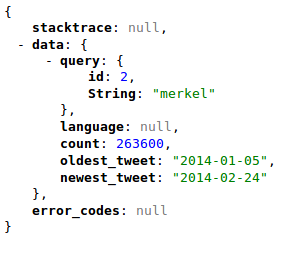
\includegraphics[scale=0.6]{Bilder/RestApi/queriesMetadata.png}
\end{figure}

\noindent
\textbf{GET \texttt{/queries/hasDaemonFetched}}
\begin{table}[h!]
\begin{tabular}{| c | p{\tweite} | l |}
\hline
	\textbf{Parameter} & \textbf{Beschreibung} &  \\
\hline \hline
 	\texttt{id} & ID eines Suchbegriffs & verpflichtend \\
\hline
\end{tabular}
\end{table}
\newline
Überprüft, ob der Daemon für den Suchbegriff mit der angegebenen \texttt{id}, Tweets gefunden hat.
\newpage

\subsection*{Result-Methoden}
\noindent
\textbf{GET \texttt{/results/tweet}}
\begin{table}[h!]
\begin{tabular}{| c | p{\tweite} | l |}
\hline
	\textbf{Parameter} & \textbf{Beschreibung} &  \\
\hline \hline
 	\texttt{id} & ID eines Tweets & verpflichtend \\
\hline
\end{tabular}
\end{table}
\newline
Liefert alle Informationen für den Tweet dieser \texttt{id} aus der Datenbank.

\noindent
\textbf{GET \texttt{/results/tweets}}
\begin{table}[h!]
\begin{tabular}{| c | p{10.1cm} | l |}
\hline
	\textbf{Parameter} & \textbf{Beschreibung} &  \\
\hline \hline
 	\texttt{id} & ID eines Suchbegriffs & verpflichtend \\
\hline
 	\texttt{sent} & Sentiment: liefert nur Tweets mit diesem Sentiment zurück, erlaubte Eingaben: "`positive"', "`neutral"', "`negative"' (alle Tweets falls nicht angegeben) & optional \\
\hline
 	\texttt{start} & Datum im Format YYYY-DD-MMTHH:MM:SS, Datum des ältesten zurückgegebenen Tweets (keine untere Grenze falls nicht angegeben) & optional \\
\hline
 	\texttt{end} & Datum im Format YYYY-DD-MMTHH:MM:SS, Datum des neuesten zurückgegebenen Tweets (keine obere Grenze falls nicht angegeben) & optional \\
\hline
 	\texttt{lang} & Sprache der Tweets im ISO-Format wie von Twitter erkannt (alle Tweets falls nicht angegeben) &  optional\\
\hline
 	\texttt{limit} & Anzahl zurückgelieferter Tweets (100 falls nicht angegeben) & optional \\
\hline
\end{tabular}
\end{table}
\newline
Liefert die Tweets, die dem Suchbegriff dieser \texttt{id} zugeordnet sind, unter den angegebenen Einschränkungen.

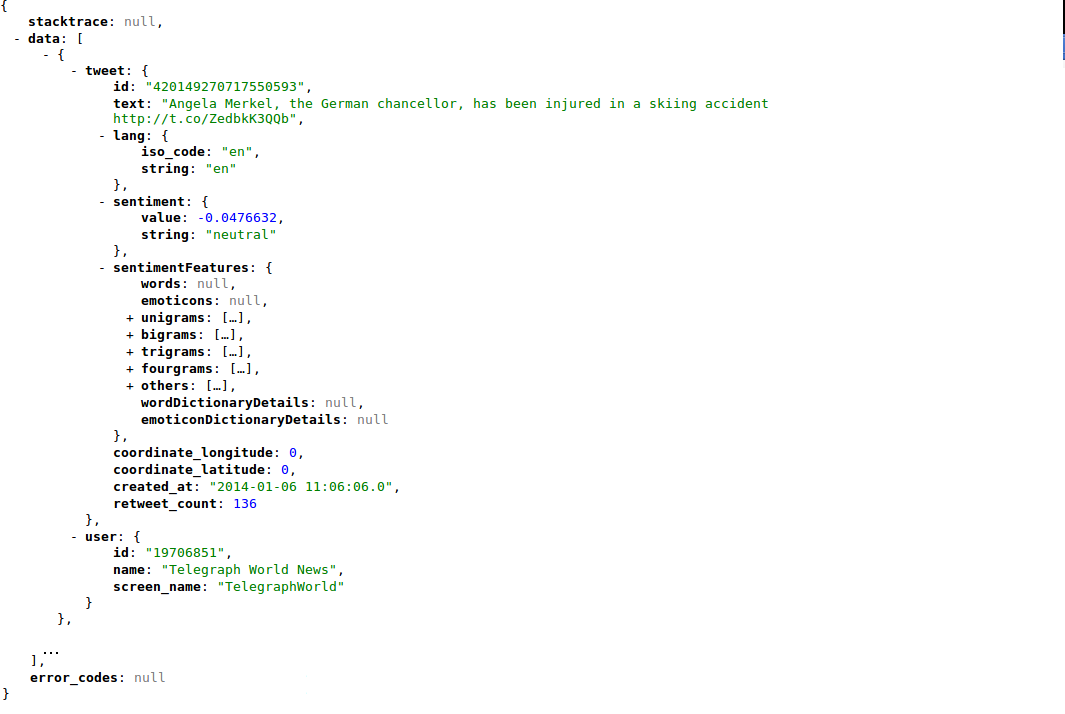
\includegraphics[scale=0.6]{Bilder/RestApi/GetTweet.png}

\noindent
\textbf{GET \texttt{/results/user}}
\begin{table}[h!]
\begin{tabular}{| c | p{\tweite} | l |}
\hline
	\textbf{Parameter} & \textbf{Beschreibung} &  \\
\hline \hline
 	\texttt{id} & ID eines Twitter-Users & verpflichtend \\
\hline
\end{tabular}
\end{table}
\newline
Liefert alle Informationen für den User dieser \texttt{id} aus der Datenbank.

\newpage
\noindent
\textbf{GET \texttt{/results/sentimentPerHour}}
\begin{table}[h!]
\begin{tabular}{| c | p{\tweite} | l |}
\hline
	\textbf{Parameter} & \textbf{Beschreibung} &  \\
\hline \hline
 	\texttt{id} & ID eines Suchbegriffs & verpflichtend \\
\hline
 	\texttt{lang} & Sprache der angezeigten Tweets (alle Tweets falls nicht angegeben) & optional \\
\hline
\end{tabular}
\end{table}
\newline
Liefert für jede volle Stunde die Anzahl positiver und negativer Posts zum Suchbegriff mit dieser \texttt{id} zurück.

\noindent
\textbf{GET \texttt{/results/countPerHour}}
\begin{table}[h!]
\begin{tabular}{| c | p{\tweite} | l |}
\hline
	\textbf{Parameter} & \textbf{Beschreibung} &  \\
\hline \hline
 	\texttt{id} & ID eines Suchbegriffs & verpflichtend \\
\hline
 	\texttt{lang} & Sprache der angezeigten Tweets (alle Tweets falls nicht angegeben) & optional \\
\hline
\end{tabular}
\end{table}
\newline
Liefert für jede volle Stunde die Anzahl Posts zum Suchbegriff mit dieser \texttt{id} zurück.

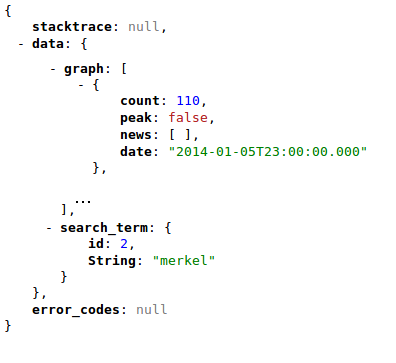
\includegraphics[scale=0.6]{Bilder/RestApi/resultsCountPerHour.png}

\newpage
\noindent
\textbf{GET \texttt{/results/tagCloud}}
\begin{table}[h!]
\begin{tabular}{| c | p{\tweite} | l |}
\hline
	\textbf{Parameter} & \textbf{Beschreibung} &  \\
\hline \hline
 	\texttt{id} & ID eines Suchbegriffs & verpflichtend \\
\hline
 	\texttt{lang} & Sprache der angezeigten Tweets (alle Tweets falls nicht angegeben) & optional \\
\hline
 	\texttt{count} &  Anzahl einbezogener Tweets (100 falls nicht angegeben) & optional \\
\hline
\end{tabular}
\end{table}
\newline
Liefert den konkatenierten Text der festgelegten Anzahl Tweets zum Suchbegriff der angegebenen \texttt{id} zurück, sodass damit auf Client-Seite die Tag-Cloud erstellt werden kann.

\noindent
\textbf{GET \texttt{/results/sentiments}}
\begin{table}[h!]
\begin{tabular}{| c | p{\tweite} | l |}
\hline
	\textbf{Parameter} & \textbf{Beschreibung} &  \\
\hline \hline
 	\texttt{id} & ID eines Suchbegriffs & verpflichtend \\
\hline
 	\texttt{lang} & Sprache der angezeigten Tweets (alle Tweets falls nicht angegeben) & optional \\
\hline
\end{tabular}
\end{table}
\newline
Durchsucht die Tweets zum Suchbegriff mit der angegebenen \texttt{id} und liefert zurück, wieviele von ihnen jeweils das Sentiment "`positiv"', "`neutral"' und "`negativ"' haben.
\begin{figure}[h!]
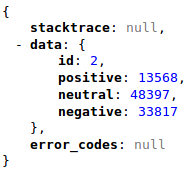
\includegraphics[scale=0.6]{Bilder/RestApi/resultsSentiment.png}
\end{figure}

\noindent
\textbf{GET \texttt{/results/getDataGroups}}
\begin{table}[h!]
\begin{tabular}{| c | p{\tweite} | l |}
\hline
	\textbf{Parameter} & \textbf{Beschreibung} &  \\
\hline \hline
 	\texttt{id} & ID eines Suchbegriffs & verpflichtend \\
\hline
 	\texttt{lang} & Sprache der angezeigten Tweets (alle Tweets falls nicht angegeben) & optional \\
\hline
\end{tabular}
\end{table}
\newline
Durchsucht die Tweets zum Suchbegriff mit der angegebenen \texttt{id} und liefert zurück, welcher Tweet zu welchem Cluster gehört.

\newpage
\noindent
\textbf{GET \texttt{/results/peaks}}
\begin{table}[h!]
\begin{tabular}{| c | p{\tweite} | l |}
\hline
	\textbf{Parameter} & \textbf{Beschreibung} &  \\
\hline \hline
 	\texttt{id} & ID eines Suchbegriffs & verpflichtend \\
\hline
 	\texttt{lang} & Sprache der angezeigten Tweets (alle Tweets falls nicht angegeben) & optional \\
\hline
\end{tabular}
\end{table}
\newline
Liefert die Peaks des Suchbegriffs dieser \texttt{id} zurück.

\noindent
\textbf{GET \texttt{/results/news}}
\begin{table}[h!]
\begin{tabular}{| c | p{\tweite} | l |}
\hline
	\textbf{Parameter} & \textbf{Beschreibung} &  \\
\hline \hline
 	\texttt{id} & ID eines Suchbegriffs & verpflichtend \\
\hline
 	\texttt{lang} & Sprache der angezeigten Tweets (alle Tweets falls nicht angegeben) & optional \\
\hline
 	 \texttt{day} &  Tag für den die News abzufragen sind & optional \\
\hline
 	 \texttt{month} & Monat für den die News abzufragen sind & optional \\
\hline
 	 \texttt{year} & Jahrg für den die News abzufragen sind & optional \\
\hline
\end{tabular}
\end{table}
\newline
Liefert die News des Suchbegriffs dieser \texttt{id} für den angegebenen Zeitraum zurück:
\begin{figure}[h!]
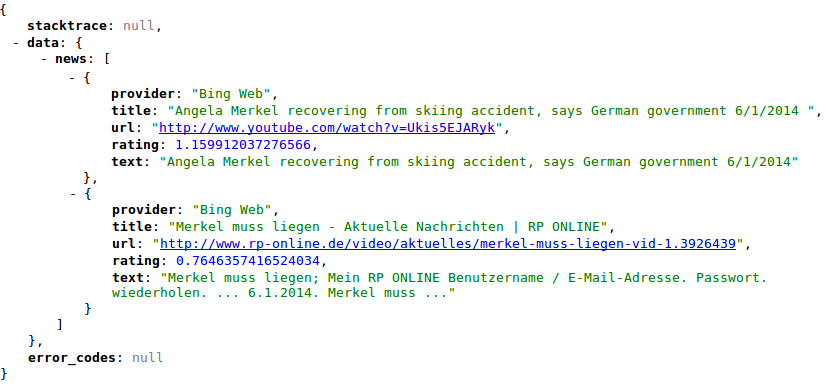
\includegraphics[scale=0.6]{Bilder/RestApi/resultNews.png}
\end{figure}

\newpage
\noindent
\textbf{GET \texttt{/results/languages}}
\begin{table}[h!]
\begin{tabular}{| c | p{\tweite} | l |}
\hline
	\textbf{Parameter} & \textbf{Beschreibung} &  \\
\hline \hline
 	\texttt{id} & ID eines Suchbegriffs & verpflichtend \\
\hline
\end{tabular}
\end{table}
\newline
Gibt eine Liste von Sprachen zurück (eine Sprache besteht aus isoCode und Häufigkeit).

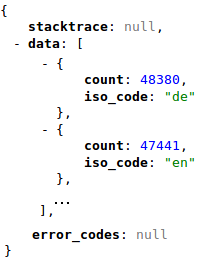
\includegraphics[scale=0.6]{Bilder/RestApi/resultLanguages.png}

\noindent
\textbf{GET \texttt{/results/trainingTweets}}
\begin{table}[h!]
\begin{tabular}{| c | p{\tweite} | l |}
\hline
	\textbf{Parameter} & \textbf{Beschreibung} &  \\
\hline \hline
 	\texttt{feature} & Betrachtetes Feature & verpflichtend \\
\hline
 	\texttt{lang} & Sprache des Modells & optional \\
\hline
\end{tabular}
\end{table}
\newline
Gibt eine Liste von Tweets zurück, die das angegebene Feature für die spezifizierte Sprache am meißten beeinflusst haben.

\noindent
\textbf{GET \texttt{/results/hashtagstatistics}}
\begin{table}[h!]
\begin{tabular}{| c | p{\tweite} | l |}
\hline
	\textbf{Parameter} & \textbf{Beschreibung} &  \\
\hline \hline
 	\texttt{id} & ID eines Suchbegriffs & verpflichtend \\
\hline
 	\texttt{lang} & Sprache der angezeigten Tweets (alle Tweets falls nicht angegeben) & optional \\
\hline
\end{tabular}
\end{table}
\newline
Durchsucht die Tweets zum Suchbegriff mit der angegebenen \texttt{id} und liefert zurück, welcher Hashtags darin vorkommen. Die Ausgabe ist sortiert nach den Häufigkeiten.
\begin{figure}[h!]
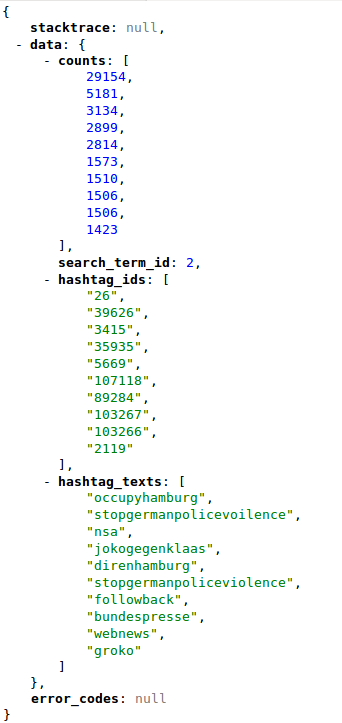
\includegraphics[scale=0.6]{Bilder/RestApi/resultsHashtagStatistics.png}
\end{figure}